\chapter{Evaluación Segundo Parcial}
\newpage
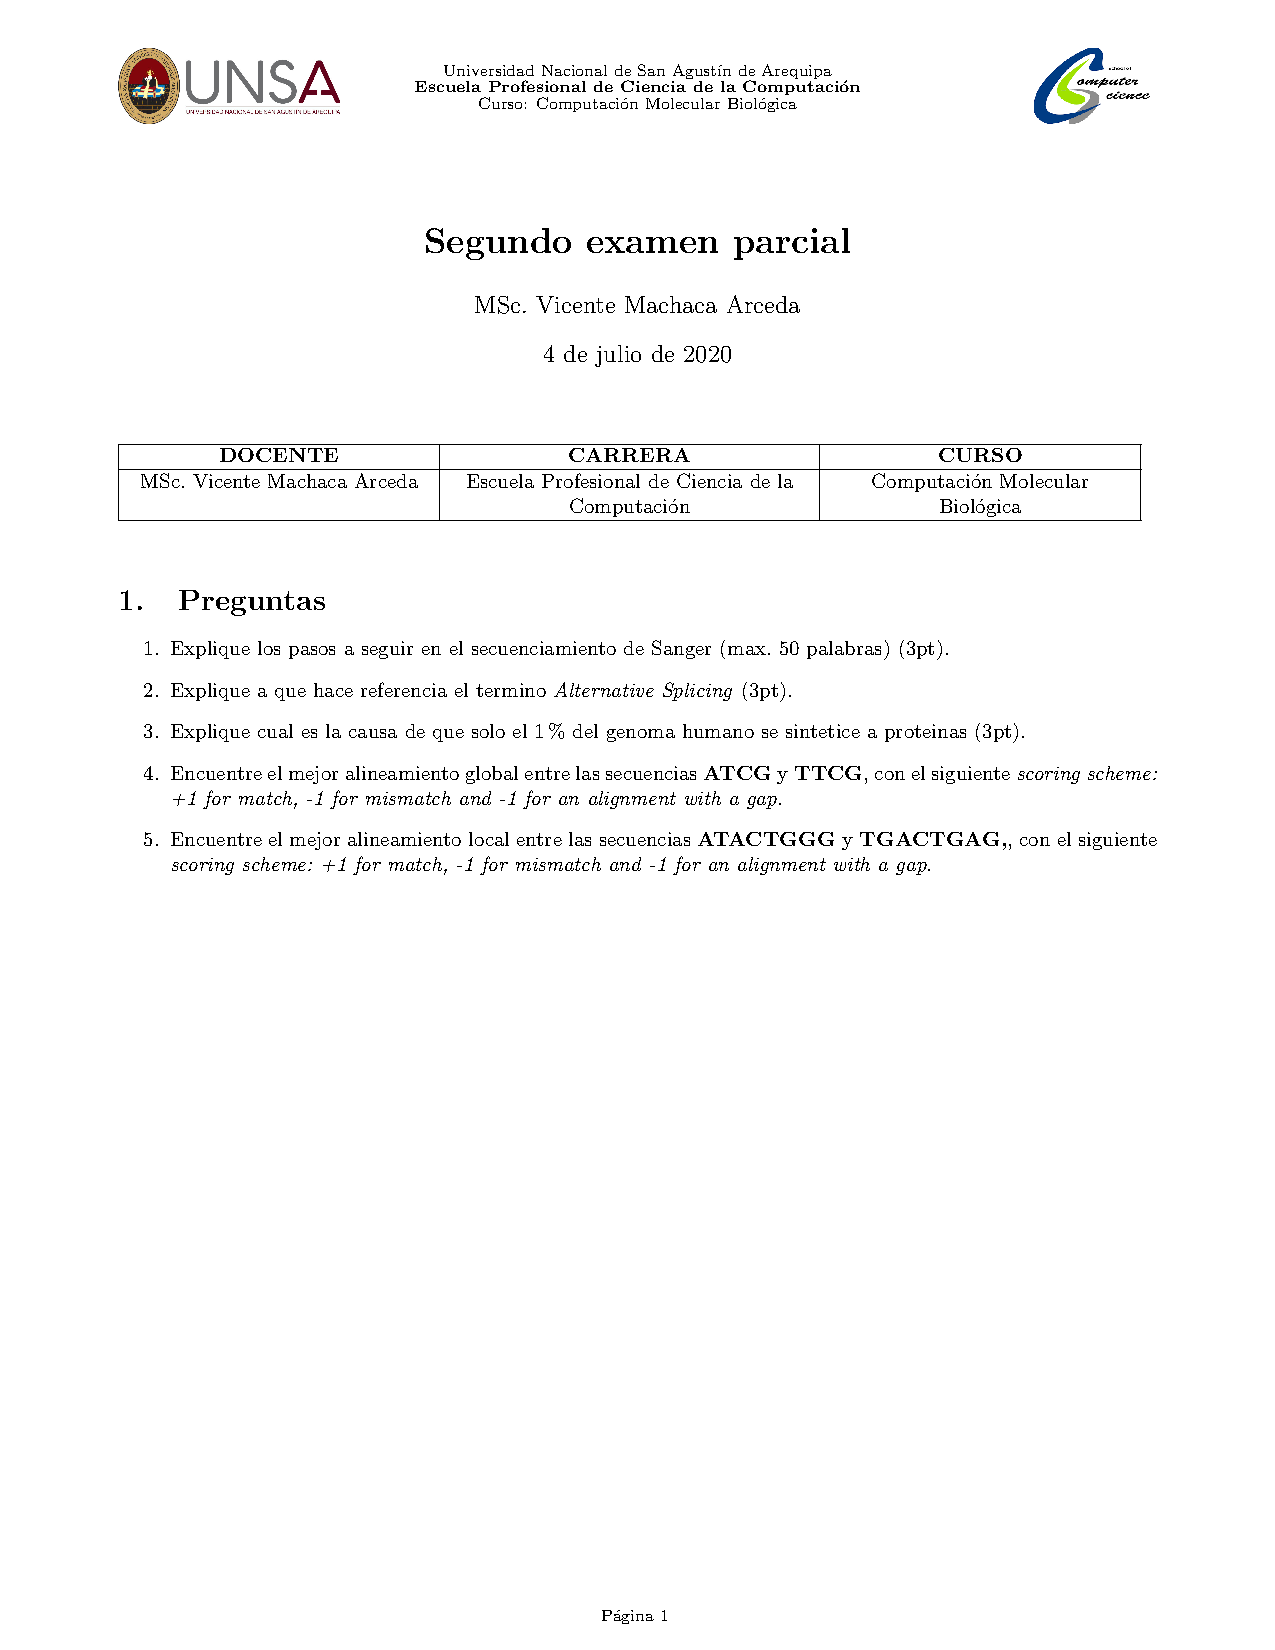
\includepdf[pages={1-}]{pdfs/examen_2.pdf}
%\includepdf[pages={1-}]{pdfs/examen_2_sol.pdf}
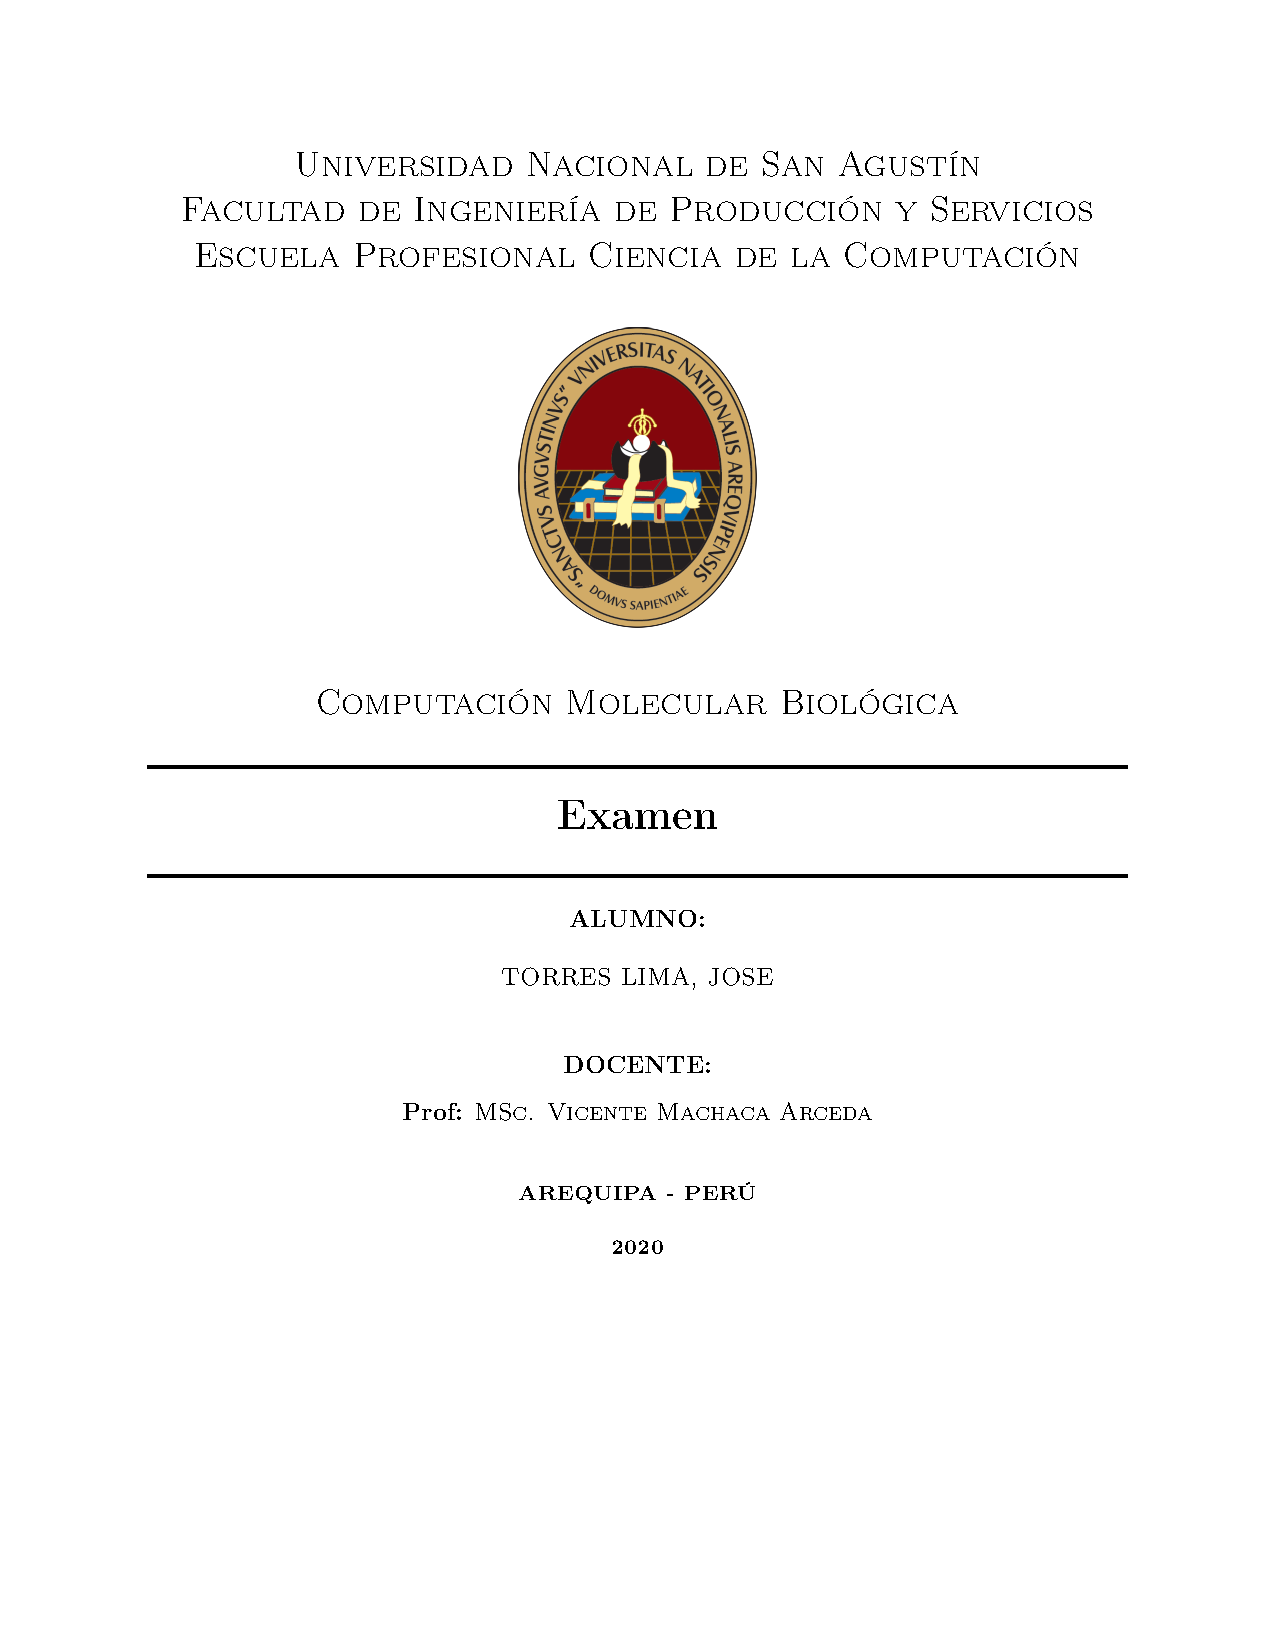
\includepdf[pages={1-}]{pdfs/examen_2_best.pdf}
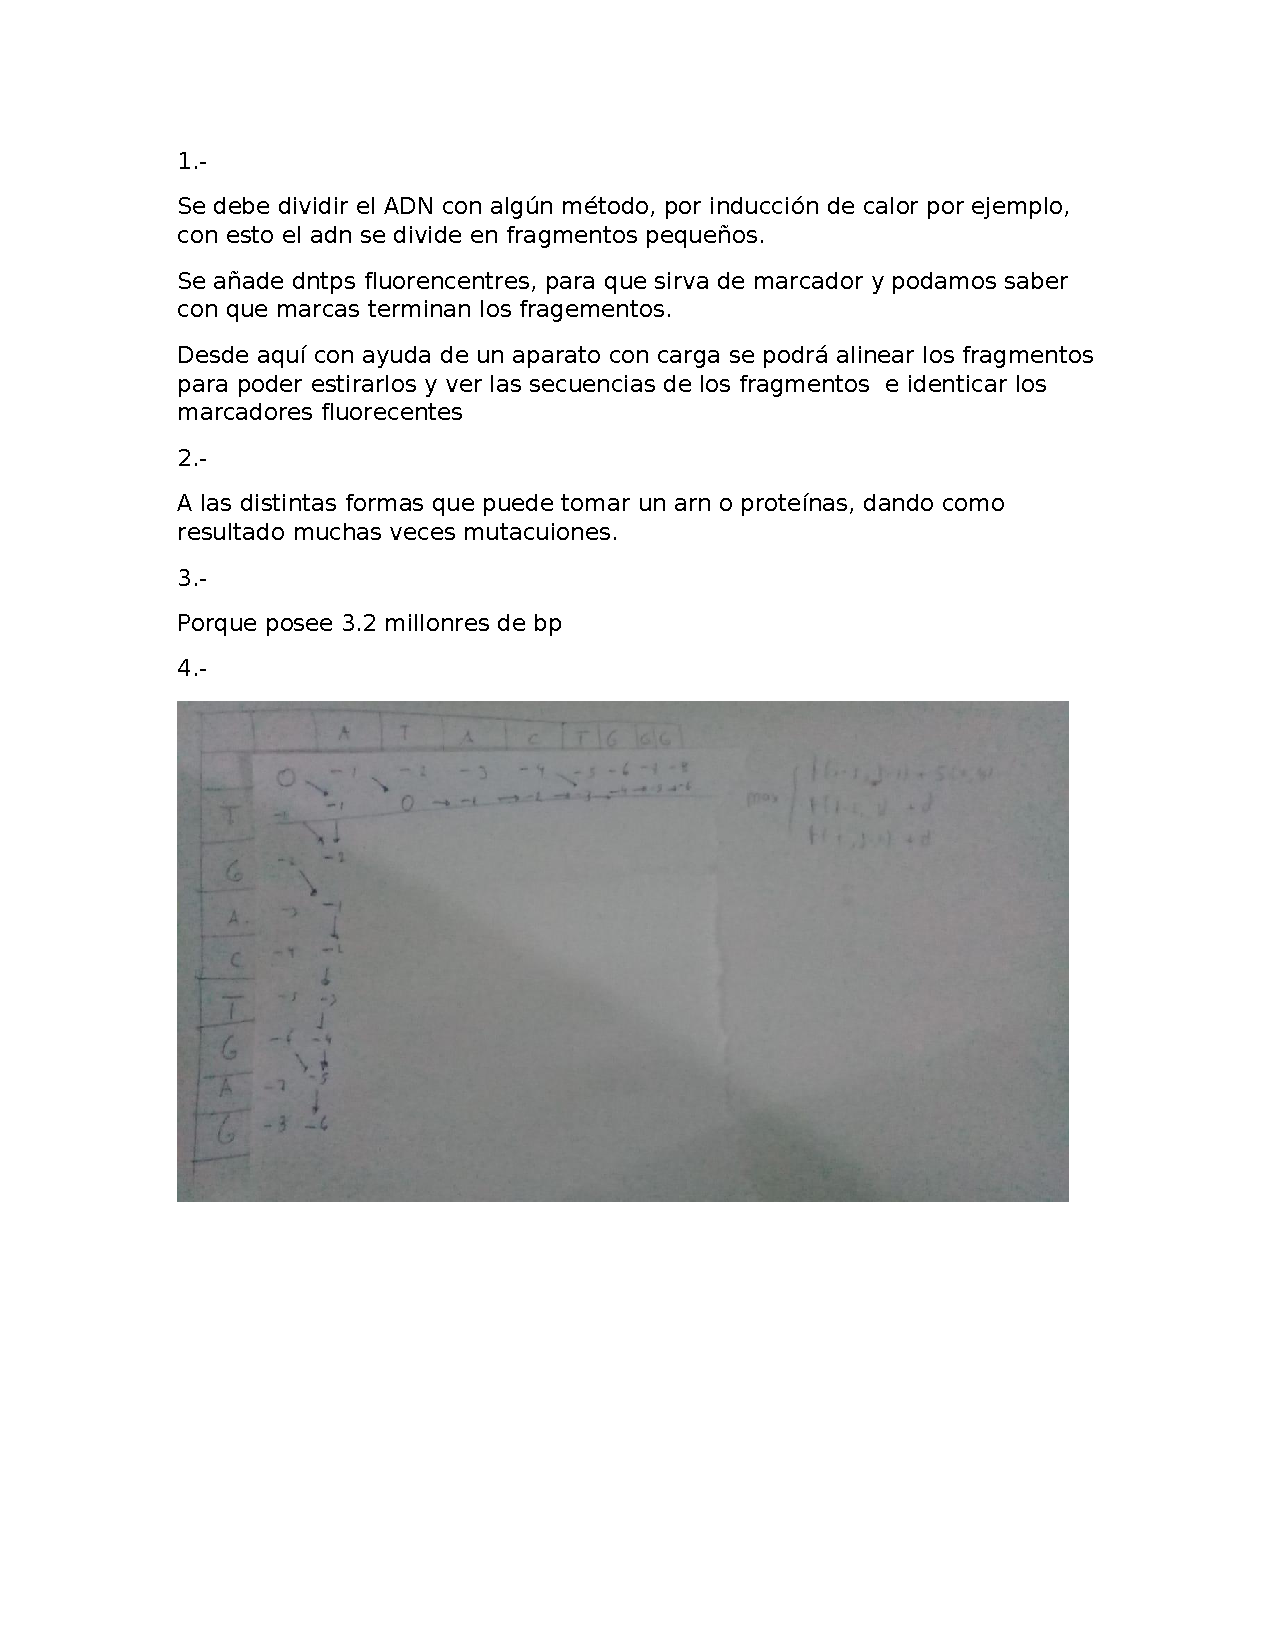
\includepdf[pages={1-}]{pdfs/examen_2_worst.pdf}

\pagestyle{empty} % Disable headers and footers for the following pages

\section{Evidencias}
Rindieron la Primera Evaluación Parcial 16 estudiantes de los 17 estudiantes matriculados, lo que representa un 100.0\%.

La nota promedio de los estudiantes que rindieron la Primera Evaluación Parcial es 10 puntos. Las notas y la evidencia de la Primera Evaluación Parcial se encuentran en la siguiente tabla:


\begin{table}[h]
\centering
\begin{tabular}{l|c|c}
\hline
\textbf{Apellidos y Nombres} & 
\textbf{Nota} & 
\textbf{Evidencia} 
\\ \hline
Amable Romero, Diego Javier &
18.0 &
\href{https://drive.google.com/open?id=1pMWVNwmbCAlMKkkZ20HA2tJ4Cz9KOybp}{Link}
\\ \hline
Bernal Chahuayo, Luis Antonio &
14.0 &
\href{https://drive.google.com/open?id=177e8FGFaXUCIT2CRNO_i-DiU06sjkQH7}{Link}
\\ \hline
Caceres Zegarra, Luis Gustavo &
15.5 &
\href{https://drive.google.com/open?id=1eVcAY1rwdjbxuOwQviGR0tYqKSX-VrGD}{Link}
\\ \hline
Espinel Quispe, Ingrid Sally &
04.5 &
\href{https://drive.google.com/open?id=1tdDHdv3b46FVcuoXfkDbHvityP70oWh7}{Link} 
\\ \hline
Gordillo Viña, Karen &
15.0 &
\href{https://drive.google.com/open?id=1ecqq7fwLKZL_8FLpzCGptllY4I3oc1so}{Link}
\\ \hline
Gutierrez Salazar, Enrique Alonzo &
18.7 &
\href{https://drive.google.com/open?id=1qV4qk05ky-xGPGJethajAdj1_zb7YUtA}{Link}
\\ \hline
Hancco Tancayllo, Hermith &
13.7 &
\href{https://drive.google.com/open?id=1_YK49t-_ge6nm_LrBNI-0m6FXANRIxAt}{Link}
\\ \hline
Huaman Canqui Jair, Francesco &
15.5 &
\href{https://drive.google.com/open?id=1-OCEerOcv43sP_aU34rc4MLzQVfceVqZ}{Link}
\\ \hline
Lacuaña Apaza, Margarita &
10.3 &
\href{https://drive.google.com/open?id=1tQUwWS700bsLdf5w4zHMgHvI45HGMaNF}{Link}
\\ \hline
Larraondo Lancho, Alejandro Jesús &
18.7 &
\href{https://drive.google.com/open?id=1gHoNNeh1olKAMd4VEmBgero5vv3do5KI}{Link}
\\ \hline
Mamani Chirinos, Luis &
05.7 &
\href{https://drive.google.com/open?id=1HS19DQegS3izRw6_yOG-zwSM13TGqBIq}{Link}
\\ \hline
Mendoza Villarroel, Alexis &
19.0 &
\href{https://drive.google.com/open?id=1V_T9FFp58mzFjYLbZTlKu7S_lvrgFJe1}{Link}
\\ \hline
Quincho Mamani, Lehi &
09.2 &
\href{https://drive.google.com/open?id=1c6taLWJSFkWHZmj0zQziyrWUinz3-A8m}{Link}
\\ \hline
Quispe Quicano, Julio Cesar &
11.7 &
\href{https://drive.google.com/open?id=1BapaIzxoX-3Nd3rEekwmFkYuOK9pmUPo}{Link}
\\ \hline
Turpo Apaza, Crhistian Andrew &
17.7 &
\href{https://drive.google.com/open?id=1Fg3SU_YOXJaY4Mqb28qrCIKOdIdZHix4}{Link}
\\ \hline
Uñapilco Chambi, Katherin &
15.7 &
\href{https://drive.google.com/open?id=16Cp0sT3WmDwVarLYgWCnLJX9JISUqpoc}{Link}
\\ \hline
\end{tabular}
\caption{Resultados Segunda Evaluación Parcial}
\label{tab:evalucion_parcial_2} % Unique label used for referencing the table in-text
%\addcontentsline{toc}{table}{Table \ref{tab:example}} % Uncomment to add the table to the table of contents
\end{table}
%------------------------------------------------
